
\begin{minipage}[t]{1.0\linewidth}

\begin{center}
\vspace{2em}

{\Huge \textbf Taylor Swift}


{\large Student device registration}
\end{center}

\begin{center}
\fbox{
\includegraphics[scale=0.3]{figure/qr-student-image.png}}

{\large Scan this code to be directed} \\
{\large to the page to register} \\
{\large your own device.} \\
\end{center}
\vspace{4em}

\normalsize
\begin{center}
% ----------------------------------
\begin{minipage}[t]{0.24\linewidth}
\fbox{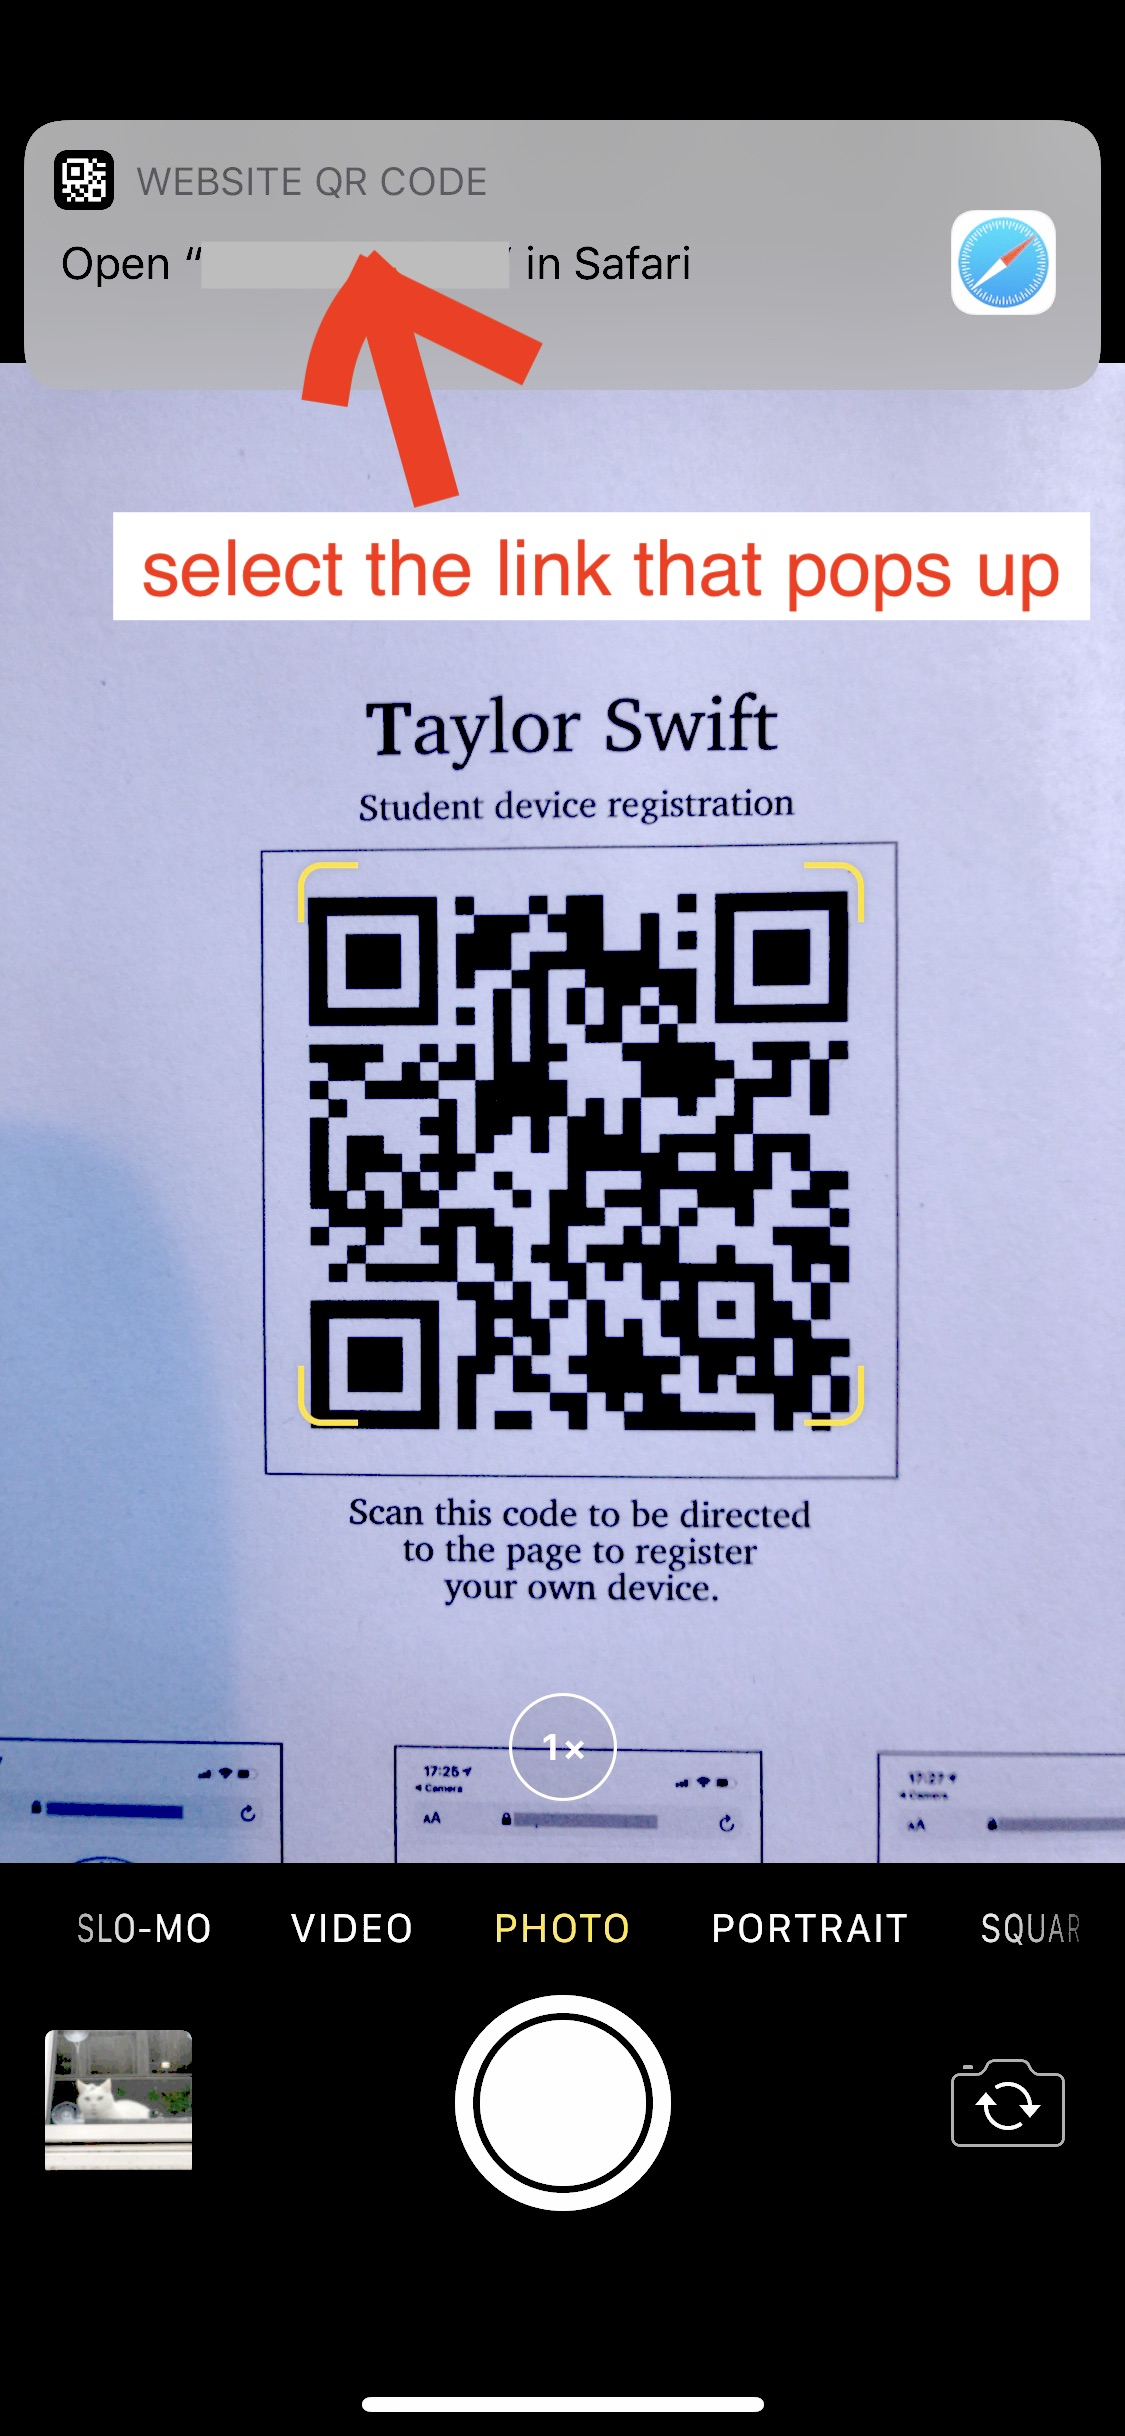
\includegraphics[scale=0.1]{figure/workflow-reg-iphone-scan.jpeg}}

Check your browser is \emph{not} in private mode, then show the QR code
to your camera app. A link should pop up once the camera sees the code.
\end{minipage}
\hspace{3em}
% ----------------------------------
\begin{minipage}[t]{0.24\linewidth}
\fbox{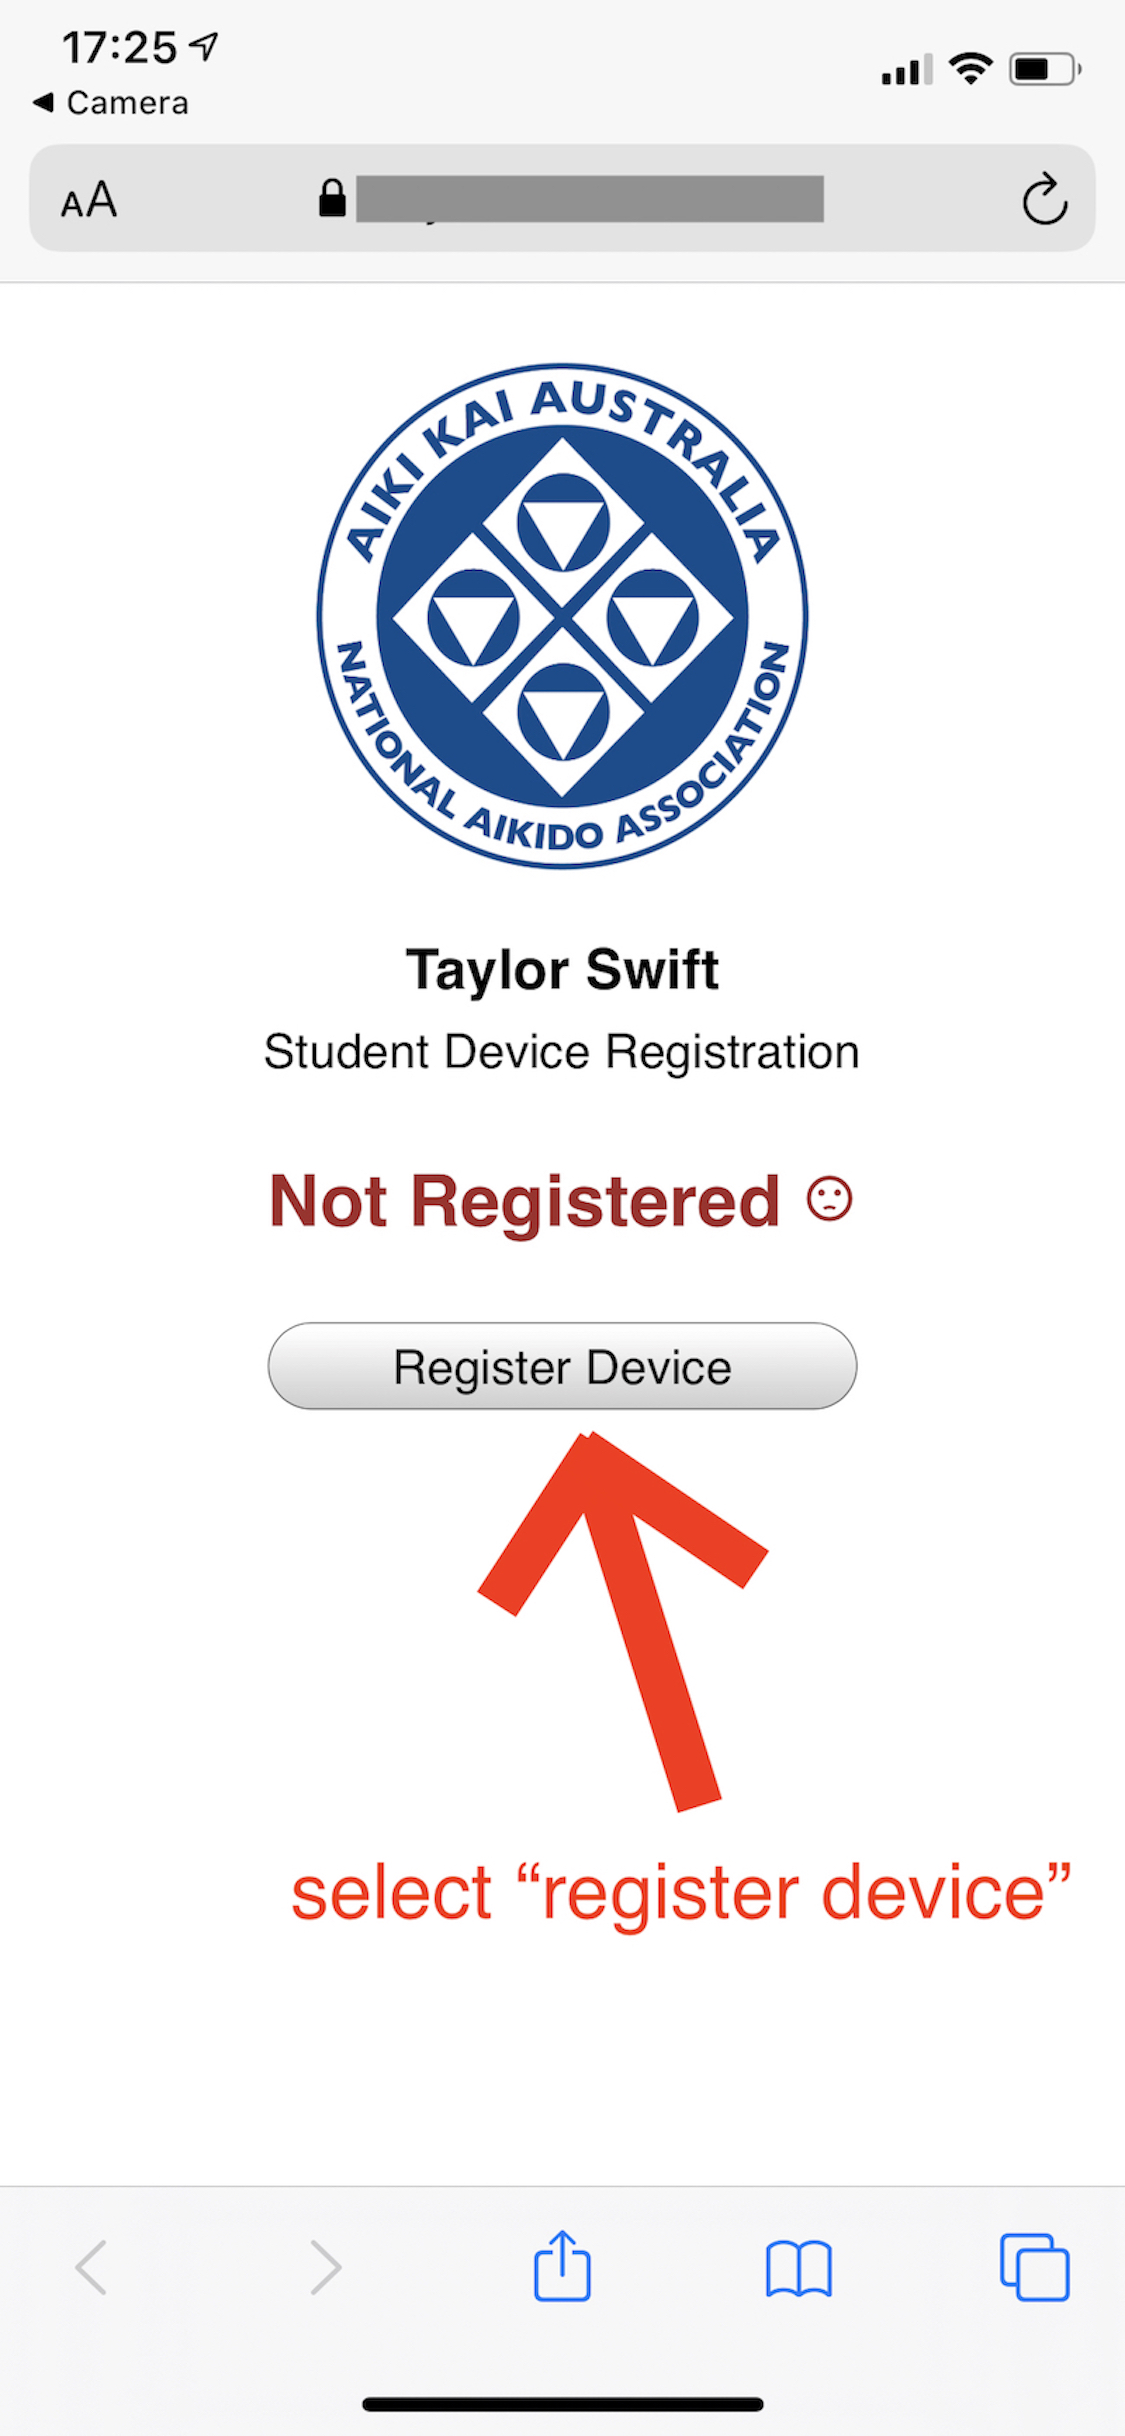
\includegraphics[scale=0.1]{figure/workflow-reg-iphone-unreg.jpeg}}

Selecting the link should direct
you to a page with your own name.
This is not the same as taking a photo of the code.
\end{minipage}
\hspace{3em}
% ----------------------------------
\begin{minipage}[t]{0.24\linewidth}
\fbox{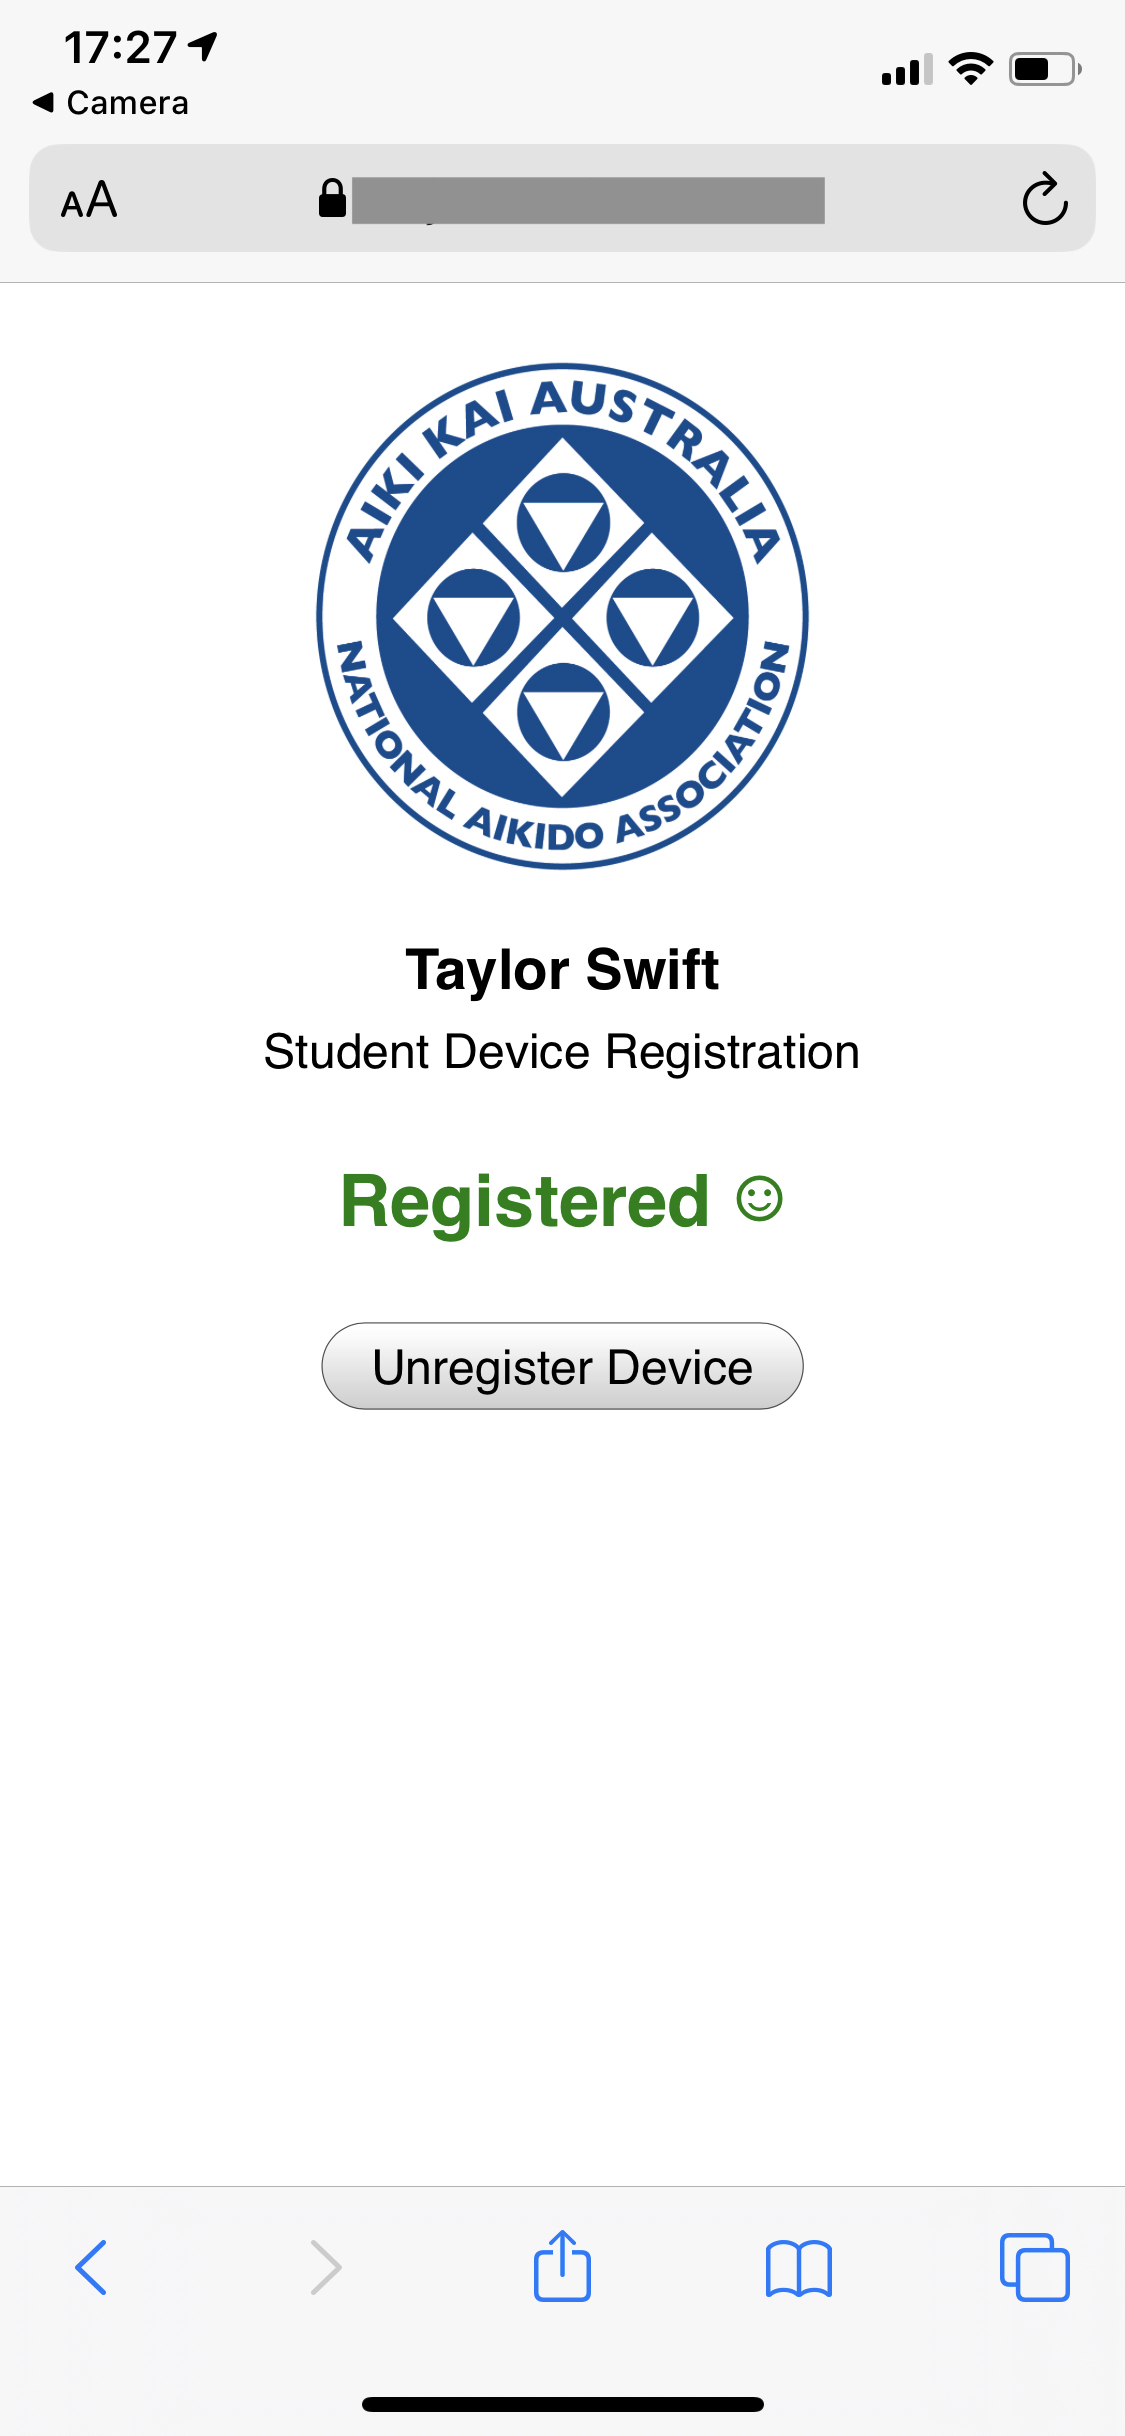
\includegraphics[scale=0.1]{figure/workflow-reg-iphone-reg.jpeg}}

Select the button to register or unregister your phone.
The page says "registered" when the server can detect
your identification cookie.

\end{minipage}
\end{center}

\end{minipage}